\section{Evaluation and Discussion}
\label{sec:ch2:results}

\begin{figure*}[t]
\centering
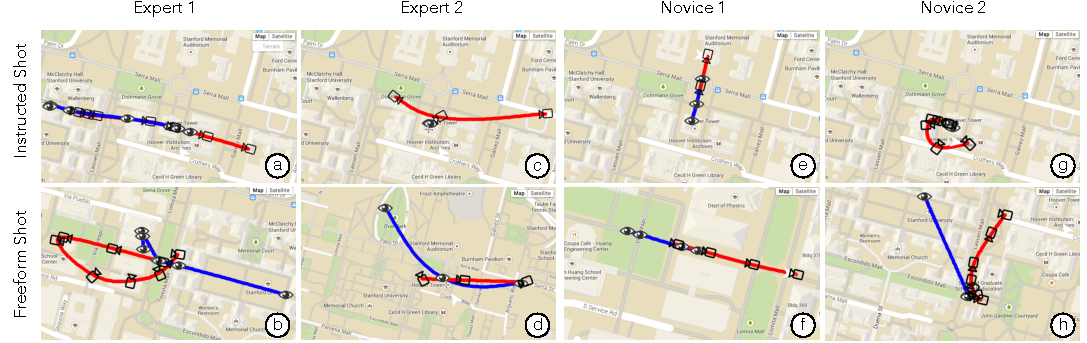
\includegraphics[width=6.0in]{images/2015_siggraph_asia/eval_trajectories.pdf}
\caption{
Camera shots created by the two experts (left) and two novices (right) in our user study.
%The top row shows each user's instructed shot the shots of Hoover Tower they were instructed to create. The bottom row shows the freeform shots they created.
The look-from and look-at trajectories for each shot are shown in red and blue respectively. The shots created by our participants contain a wide variety of camera motions.
}
\label{fig:ch2:all_shots}
\end{figure*}

In this section, we describe the user study we conducted to evaluate our tool, and discuss our key findings.

\paragraph{User Study}

We performed a user study aiming to understand whether our tool enables the creation of shots that would be challenging to capture otherwise.
We recruited two expert cinematographers, and two novice cinematographers with computer graphics experience. Both of our expert cinematographers had extensive experience manually flying quadrotors for cinematography.

After demonstrating the capabilities of our tool in a 30 minute tutorial, we gave all four participants identical tasks.
We first tasked them with creating one shot featuring the 285 foot tall Hoover Tower (i.e., the \emph{instructed shot}).
The tower was selected for its striking appearance and large scale, providing an opportunity for interesting shots that are well-suited for quadrotor cinematography.
We also tasked participants with creating a second shot of their own choosing (i.e., the \emph{freeform shot}).
We instructed them to create and refine shots that are cinematically interesting, and within the physical limits of our quadrotor hardware, as visualized in our tool.
They had 90 minutes to create these shots, during which we were available to answer questions.
Our tool saved a log and screen recording of each session.
Afterwards, they accompanied us to capture their shots, watched the resulting videos, and filled out an exit questionnaire.

All four participants successfully completed the two tasks.
We show the shots from our users in Figure~\ref{fig:ch2:all_shots}, and henceforth we refer to the shots using the lettering in this figure.
The participants' shots included a wide variety of camera motions.
None of the shots violated any of the kinematic or dynamic limits shown on the feasibility plots in our tool.
We were able to successfully capture all eight shots.
We encourage readers to watch our supplementary video, where we show these real-world shots, and the virtual previews from our tool, in a series of side-by-side comparisons.

\begin{figure}[t]
\centering
\includegraphics[width=6.0in]{images/2015_siggraph_asia/top-down-sequ.pdf}
\caption{
Novices and experts successfully designed shots with challenging camera motions using our tool.
The expert shot (top) is especially challenging to execute manually, since it requires smoothly changing the camera orientation to look down at Hoover Tower exactly as the quadrotor flies over it.
The novice shot (bottom) contains a similar camera motion.
}
\label{fig:ch2:expert_novice_comparison}
\end{figure}

\paragraph{Novices and Experts Successfully Designed Challenging Shots}
We asked the expert cinematographers to describe what elements were challenging about the shots they created, if they were to capture them with existing approaches for quadrotor cinematography.
Each expert identified camera motions in their shots that would either take many attempts, or would have to be modified to be less challenging.
We identified similar camera motions in the novice shots (see Figure~\ref{fig:ch2:expert_novice_comparison}).
We summarize the similarities between novice and expert shots as follows,

\begin{itemize}

\item
Expert shot (c) required continuous re-orientation of the camera relative to the flight path, with the look-from trajectory in red arcing away from a fixed look-at point.
We found a similar arcing motion around a fixed look-at point in novice shots (g) and (h).
This camera motion is difficult to execute manually, because it requires continuously and precisely re-orienting the camera during flight.

\item
Expert shot (a) required flying straight towards a point over a long distance, which we also found in novice shot (f).
This camera motion is difficult to execute manually, since small initial errors in the direction of flight have to be corrected, leading to visual artifacts in the resulting video.

\item
Expert shot (a) required smoothly adjusting the rate of camera re-orientation, to end at a specific orientation at a specific time.
We found this camera motion in novice shot (a).
We show these two shots in Figure~\ref{fig:ch2:expert_novice_comparison}.
This camera motion is especially difficult to execute manually.
The camera must translate towards a point while tilting down, so that the end of the tilting motion exactly coincides with being above the tower, all while approaching the tower in a straight line.
The expert that designed shot (a) remarked that executing such a shot manually would require approximately 20 attempts.

\end{itemize}

This finding suggests that users can successfully design compelling shots with challenging camera motions using our tool, regardless of their level of expertise with quadrotors.

\paragraph{Previewing Shots Visually was Useful}
Our exit survey asked participants to identify the most useful feature of our user interface, and rank the features in our user interface on a 5-point scale from \emph{not useful} to \emph{indispensable}.
Three of the four participants identified the ability to visually preview their shot as being the most useful, and all users rated this feature as a 4 or higher.
%Several participants asked about the accuracy of this preview.
Indeed, Figure~\ref{fig:ch1:teaser_ch2} shows that our visual preview accurately estimates the appearance of recorded video footage.
This finding validates our approach of enabling users to design shots visually, and highlights the importance of ensuring physical feasibility during the design process.

\begin{figure}[t]
\centering
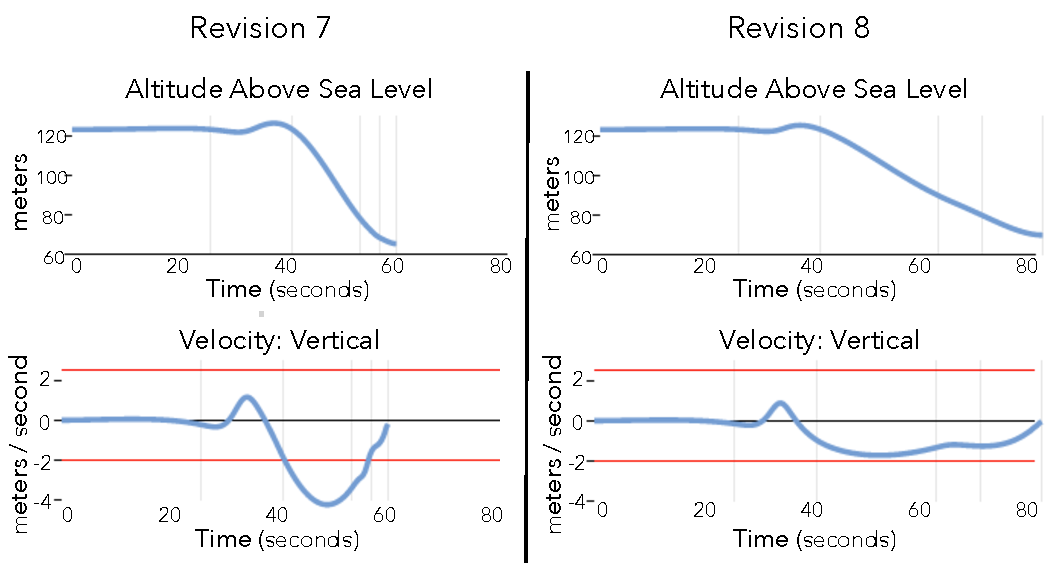
\includegraphics[width=4.0in]{images/2015_siggraph_asia/edit-infeasible.pdf}
\caption{
Participants were able to modify infeasible shots into feasible shots using the visual feedback we provide in our tool.
After his \nth{7} revision, Expert 1 found that his shot was infeasible (left).
He edited both the altitude and timing of 3 keyframes to create a feasible shot as his \nth{8} revision (right).
Horizontal red lines indicate physical limits of our quadrotor hardware.
}
\label{fig:ch2:feasibility_fix}
\end{figure}

\paragraph{Controlling the Timing of Shots was Useful}
All participants used the easing curves to refine the timing of their shots.
Participants used the easing curves to modify the pacing of their shots, and to fix feasibility violations.
In all shots, participants adjusted the default easing curve control points.
Of the eight shots created, six featured additional control points added by the participant.
This finding validates our approach of enabling users to precisely control the timing of their shots.

\paragraph{Visual Feasibility Feedback was Useful, Although Some Participants Would Have Preferred an Automatic Solution}
All of our participants responded to the visual feasibility feedback in our tool.
Users successfully modified their shots until they were within the physical limits of our hardware, as shown on the feasibility plots in our tool.
Figure~\ref{fig:ch2:feasibility_fix} shows Expert 1 modifying both the altitude and timing of three keyframes to stay within the vertical speed limit of our quadrotor.
However, participants were divided in their opinions about our feasibility plots.
One participant rated it as the best part of the tool.
He described it as essential to creating shots at the physical limits of the hardware.
Another participant expressed difficulty knowing exactly how to tweak trajectories in response to the visual feedback.
This finding suggests that some users would prefer an automatic solution for fixing feasibility issues, while others like precise control over their shots.
We believe that developing an automatic solution to fix feasibility violations is an interesting direction for future work.

\begin{tcolorbox}[before skip=20pt, after skip=20pt, sharp corners]
\begin{center}
\textbf{In Chapter~\ref{sec:ch3}, we will present an automatic algorithm for correcting feasibility violations.}
\end{center}
\end{tcolorbox}

\begin{figure}[t]
\centering
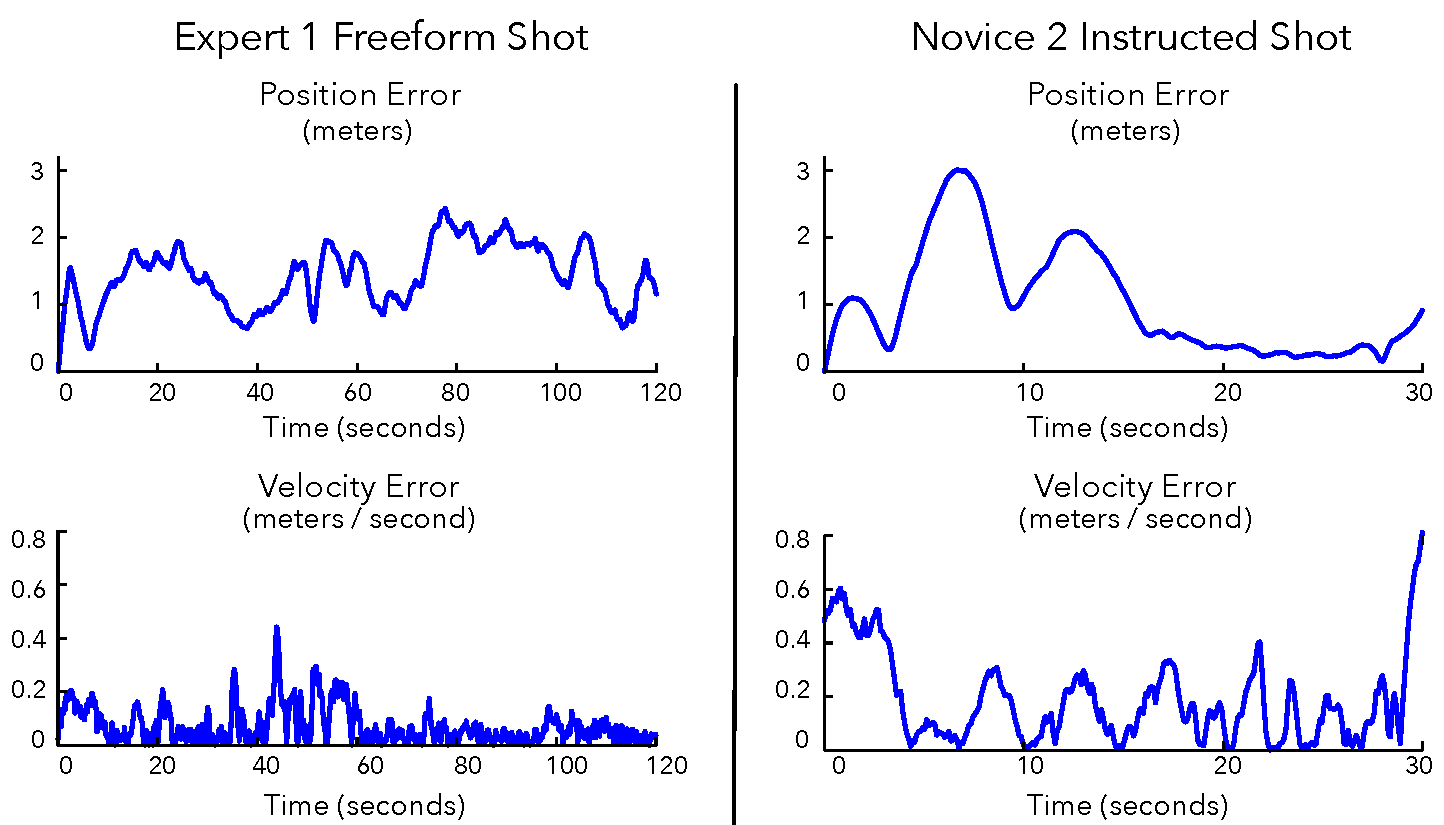
\includegraphics[width=4.0in]{images/2015_siggraph_asia/errors.pdf}
\caption{
Position and velocity error of our quadrotor for the longest (left) and shortest (right) shots.
The position error is less than 3.01m at all times, and the velocity error is less than 0.80m/s at all times.
Note that the horizontal scaling varies varies on the left and right subplots. 
}
\label{fig:ch2:errors}
\end{figure}

\paragraph{Accuracy}
To quantify how well our quadrotor camera system follows trajectories, we compared the intended trajectories created by our users, to the actual trajectories executed by our quadrotor (see Figure~\ref{fig:ch2:errors}).
The average position error across all shots was 1.12m ($\sigma = 0.57$), and was never greater than 3.01m.
The average velocity error across all shots was 0.11m/s ($\sigma = 0.10$), and was never greater than 0.80m/s.
In general, our system is limited by the positioning and pointing accuracy of our quadrotor.
This limitation makes close-up shots particularly challenging, where small errors in position lead to more noticeable visual errors.
However, our participants responded positively when they saw the captured footage for the shots they created.
This finding suggests that the level of accuracy achievable with current-generation quadrotor hardware is sufficient to obtain a variety of compelling shots.

\paragraph{Concluding Remarks}
Overall, all participants were enthusiastic about using our system.
%In particular, they remarked on the usefulness of having a 3D camera view to visualize their shot.
%Indeed, Figure~\ref{fig:teaser} shows that our visual preview accurately estimates the appearance of the recorded video footage.
Experts appreciated having a powerful tool to visually plan complex trajectories and execute repeatable takes (e.g. Expert 1 remarked \emph{``Normally I fly less ambitious paths to avoid making mistakes!''} and \emph{``I love how I can get the same shot, take after take, day after day!''}).
Novices were particularly enthusiastic about being able to capture high-quality video footage with quadrotors without having experience flying them (e.g., Novice 2 remarked, \emph{``I liked how it turned a `drone flying problem' into a `drawing a curve in space problem'. I don't know how to fly a drone and don't want to, but I find drawing in 3D very intuitive.'}').
